\section{Proposed System Architecture}

The system architecture is partitioned into four major subsystems designed to maximize data throughput and minimize stall cycles.

\subsection{SoC System Integration: The Hybrid I/O Architecture}
The CGRA IP is integrated into the Programmable Logic of the Zynq UltraScale+ platform. To overcome the common ``bottleneck black hole'' found in standard accelerator designs, this project proposes a \textbf{Hybrid I/O architecture} that decouples data and control paths:
\begin{itemize}
    \item \textbf{AXI4 Data Plane (DMA):} Facilitates high-bandwidth, burst-oriented communication with DDR4 DRAM for weight and spike streaming.
    \item \textbf{APB Control Plane (CSR):} A dedicated low-latency bus for register-mapped configuration, status monitoring, and interrupt handling, ensuring control transactions never stall the data pipeline.
\end{itemize}

\begin{figure}[ht!]
    \centering
    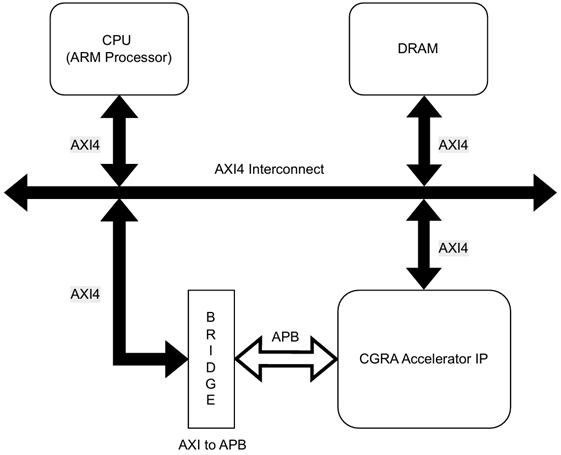
\includegraphics[width=0.8\textwidth]{images/SoC System Integration Block Diagram.png}
    \caption{Hybrid I/O Architecture: Decoupled Control (APB) and Data (AXI4) Planes}
    \label{fig:soc_integration}
\end{figure}

\subsection{Accelerator Subsystems}

\subsubsection{Global Control and CSR}
This module decodes commands from the host via the APB slave interface. It manages interrupt generation, status monitoring, and the accelerator's lifecycle.

\begin{figure}[ht!]
    \centering
    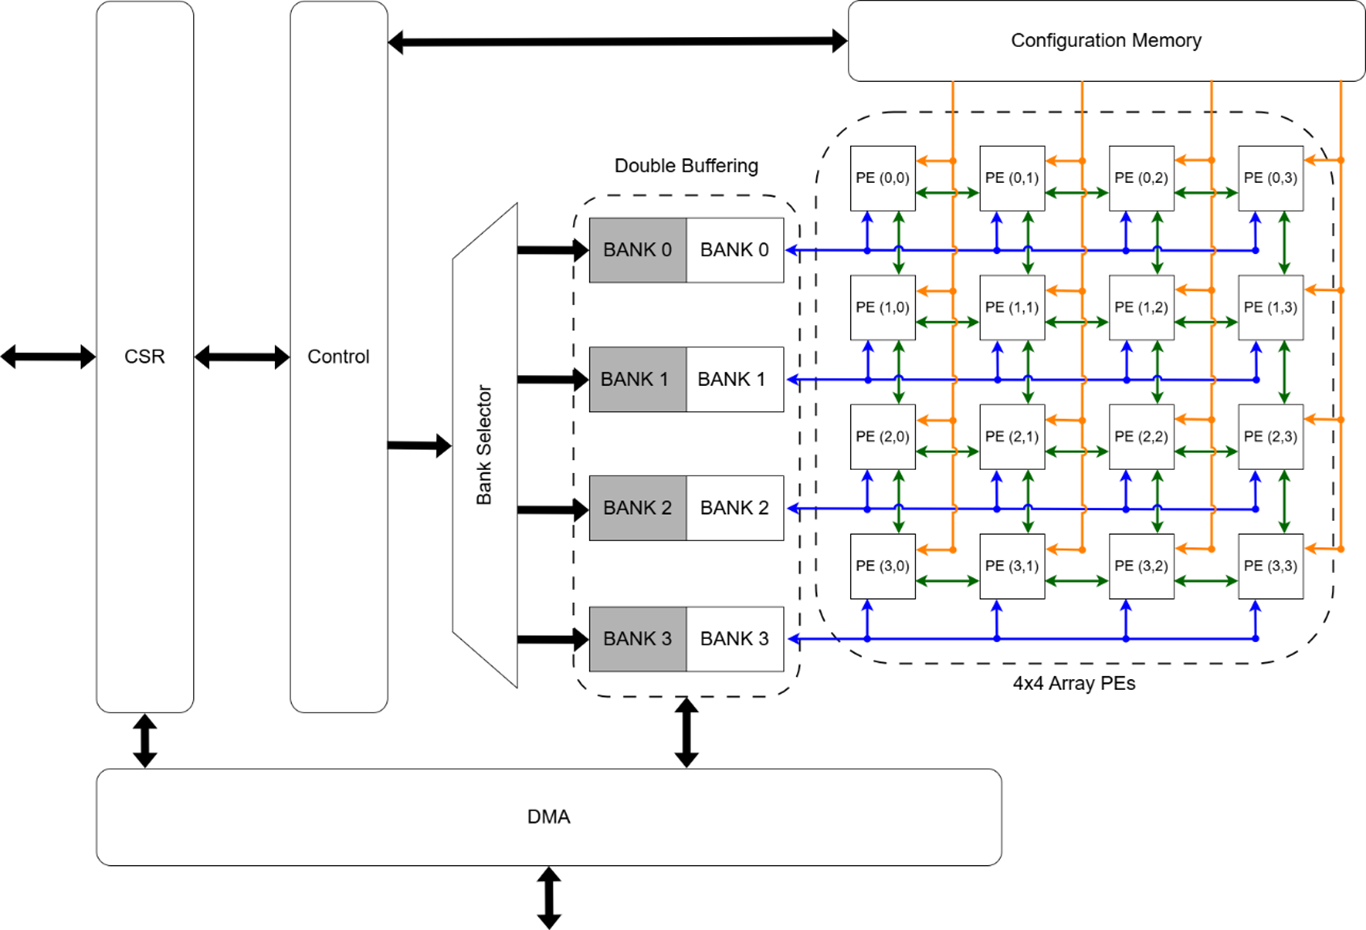
\includegraphics[width=0.8\textwidth]{images/Block Diagram for CGRA Accelerator IP.png}
    \caption{High-Level Block Diagram of the CGRA Accelerator IP Subsystems}
    \label{fig:cgra_block_diagram}
\end{figure}

\subsubsection{Double-Buffered Configuration Memory}
To support rapid reconfiguration required by multi-layer networks, the configuration memory employs a double-buffering scheme. This allows the DMA to pre-fetch the bitstream for the next layer (the ``back'' buffer) while the current layer is executing from the ``front'' buffer.

\subsubsection{Bi-Directional AXI4 DMA Engine}
The DMA unit operates as an AXI4 Master with \textbf{backpressure-aware flow control}. Unlike traditional input-only designs, this engine features a dedicated Write Engine to offload intermediate neuron states back to DDR. This enables the execution of multi-layer SNNs that exceed on-chip memory capacity without CPU-side data copying.

\begin{figure}[ht!]
    \centering
    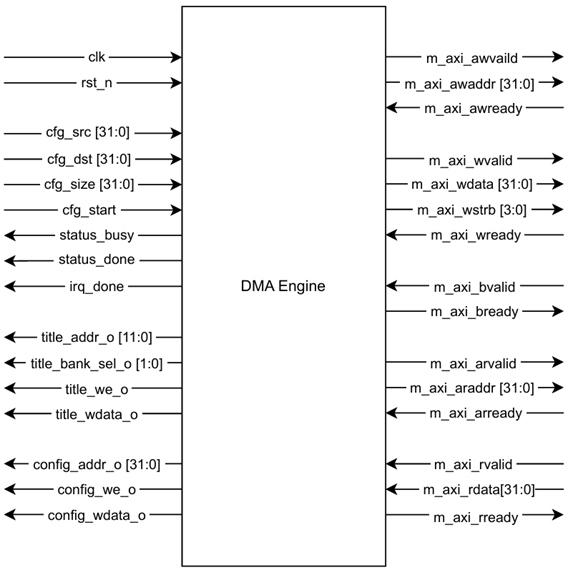
\includegraphics[width=0.8\textwidth]{images/Module DMA Engine.png}
    \caption{Bi-Directional AXI4 DMA Engine Architecture}
    \label{fig:dma_architecture}
\end{figure}

\subsubsection{Row-Banked Tile Memory}
The global tile memory is physically partitioned into four independent SRAM banks. Each bank is dedicated to a specific row of the 4×4 PE array, allowing all four rows to fetch operands simultaneously without contention.

\begin{figure}[ht!]
    \centering
    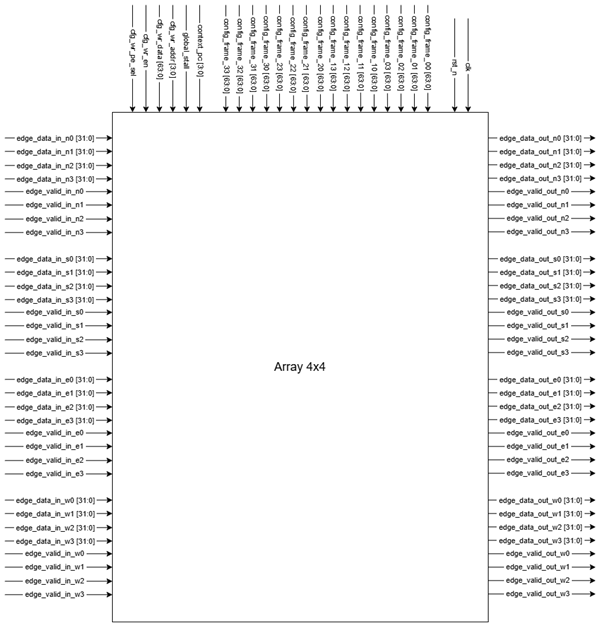
\includegraphics[width=0.7\textwidth]{images/Module Array 4x4 PEs.png}
    \caption{4x4 PE Array Mesh Topology}
    \label{fig:pe_array}
\end{figure}

\subsection{Processing Element Tile Design}
Each PE tile integrates a compute datapath, local scratchpad memory, and a \textbf{Multicast-Enabled Network-on-Chip (NoC)} router.
The PE datapath consists of:
\begin{itemize}
    \item \textbf{Decode:} Configuration frame sets opcode and route mask.
    \item \textbf{Operand Select:} Dual 4-to-1 muxes for source operand selection (RF, Neighbors, SPM, Immediate).
    \item \textbf{ALU:} 40-bit saturating MAC unit and 32-bit ALU.
    \item \textbf{LIF Unit:} Discretized neuron update logic.
    \item \textbf{Router (Multicast-Enabled NoC):} A circuit-switched mesh router. It implements a \textbf{dynamic bitmask-based multicast algorithm}, allowing a single spike packet to be replicated to any combination of North, East, South, or West neighbors in a single cycle. This is critical for SNNs with high synaptic fan-out.
\end{itemize}

\begin{figure}[ht!]
    \centering
    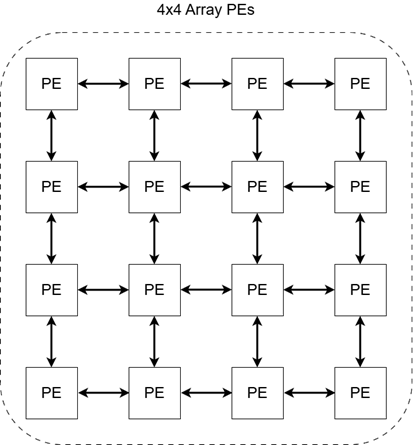
\includegraphics[width=0.8\textwidth]{images/Mesh routing for 4x4 CGRA.png}
    \caption{Multicast NoC Routing Patterns in the 4x4 Mesh}
    \label{fig:noc_routing}
\end{figure}

\subsection{Parametric Design Generation and Scalability}
To ensure the proposed architecture is not limited to a fixed 4×4 configuration, the project includes the development of a \textbf{parametric RTL generation framework}. Built using SystemVerilog parameters and Python-based templating, this framework allows for design space exploration by automatically generating NxM arrays (e.g., 8×8 or 16×16) with correctly sized NoC routing tables and DMA stride logic.
